\documentclass[11pt,a4paper,titlepage]{article}

\setlength{\oddsidemargin}{0in}
\setlength{\evensidemargin}{0in}
\setlength{\textwidth}{170mm}
\setlength{\topmargin}{-15mm}
\setlength{\textheight}{240mm}


\usepackage{hyperref}
\usepackage{listings}
\usepackage{graphicx}
\graphicspath{ {images/} }

\title{CS26020: Experimenting with Sensors}
\author{Nathan Williams - naw21}     
\date{\today}

\begin{document}
\maketitle
\tableofcontents
\listoffigures
\newpage
\section{INTRODUCTION}

\subsection{Purpose of this Document}

This document shows and discusses the result of experimenting with the IRSensors and Encoders on the Formula AllCode robots\cite{Formula all-code} and the in-robot API\cite{in-robot api}

\subsection{Objectives}
	
\begin{itemize}
	\item Collect Infrared Sensor data.
	\item Collect Encoders data
	\item Visualize the data.
	\item Analyze and discuss the data.
\end{itemize}

\section{Infrared Sensors}
\subsection{Programming}
To get the Sensor reading from the robot I wrote a function to display the data on screen.
\begin{lstlisting}[language=C,frame=single]
void IRSensors(){
 double IRDataSum[8] = {0,0,0,0,0,0,0,0};
 int j;
 for(j =0;j<10;j++){
  int i;
  for(i=0;i<8;i++){
	IRDataSum[i]=IRDataSum[i]+FA_ReadIR(i);	
  }
 }
 double IRDataAverage[8];
 int i;
 for(i=0;i<8;i++){
  IRDataAverage[i]=IRDataSum[i]/10.0;
  if (IRDataAverage[i]>600) {
   FA_LEDOn(i);
  } else {
   FA_LEDOff(i);
  }
 }
 FA_LCDClear();
 FA_LCDNumber(IRDataAverage[IR_RIGHT],0,12,FONT_NORMAL,LCD_OPAQUE);
 FA_LCDNumber(IRDataAverage[IR_REAR_RIGHT],0,1,FONT_NORMAL,LCD_OPAQUE);
 FA_LCDNumber(IRDataAverage[IR_REAR] 40,1,FONT_NORMAL,LCD_OPAQUE);
 FA_LCDNumber(IRDataAverage[IR_REAR_LEFT],80,1 ,FONT_NORMAL,LCD_OPAQUE);
 FA_LCDNumber(IRDataAverage[IR_LEFT],80,12,FONT_NORMAL,LCD_OPAQUE);
 FA_LCDNumber(IRDataAverage[IR_FRONT_LEFT],80,20,FONT_NORMAL,LCD_OPAQUE);
 FA_LCDNumber(IRDataAverage[IR_FRONT],40,20,FONT_NORMAL,LCD_OPAQUE);
 FA_LCDNumber(IRDataAverage[IR_FRONT_RIGHT],0,20,FONT_NORMAL,LCD_OPAQUE);
 FA_DelayMillis(100);
}

\end{lstlisting}

\subsection{Data Acquistion}
\subsection{Data Captured}
\subsection{Data Visualised}

\subsection{Discussion}

\section{Encoders}
\subsection{Programming}
\begin{lstlisting}[language=C,frame=single]
void encodersDataGathering(int power){
	FA_SetMotors(power,power);
	FA_DelayMillis(500 + power*10);
	int i;
	for(i = 0,i<5,i++){
		FA_ResetEncoders();
		FA_DelayMillis(1000);
		FA_LCDNumber(FA_ReadEncoder(1), 20*power, 
			1, FONT_NORMAL, LCD_OPAQUE);
		FA_LCDNumber(FA_ReadEncoder(0), 20*power, 
			12, FONT_NORMAL, LCD_OPAQUE);
	}
}

int main(){
	FA_RobotInit();
	FA_LCDBacklight(50);
	int power = 0;
	
	while(1){  
		if(FA_ReadSwitch(0)){
			FA_LCDClear();
			encodersDataGathering(power);
		}
		if(FA_ReadSwitch(1)){
			power++;
			FA_DelayMillis(200);
		}
	}
}

\end{lstlisting}
\subsection{Data Acquistion}
\subsection{Data Captured}
\subsection{Data Visualised}
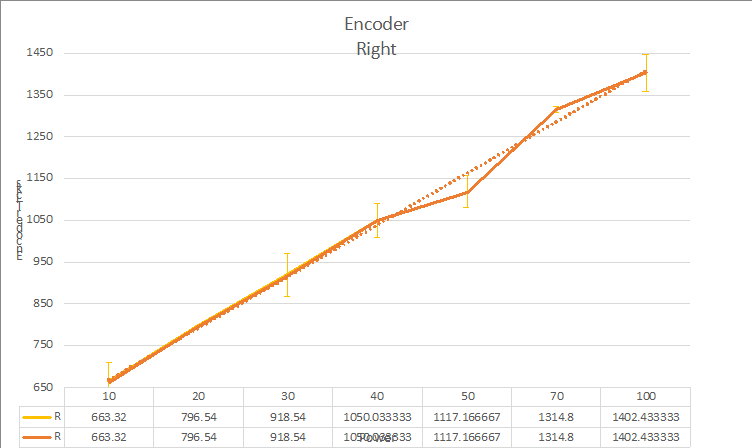
\includegraphics{EncodersRight}

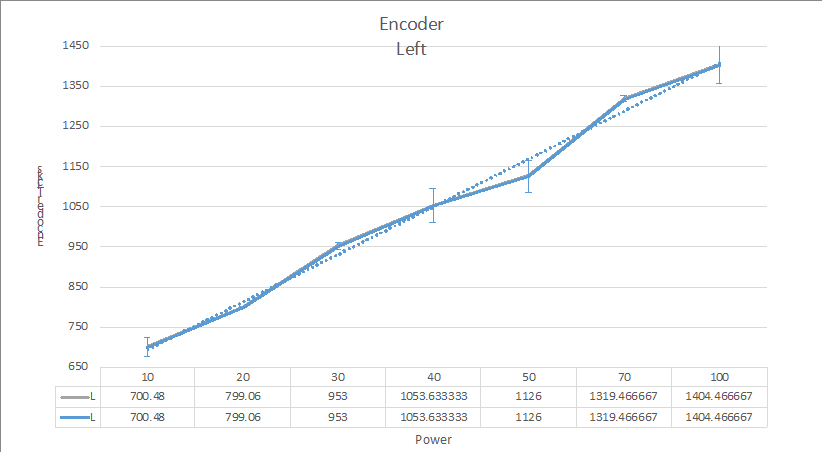
\includegraphics{EncodersLeft}
\subsection{Discussion}

\clearpage
\addcontentsline{toc}{section}{REFERENCES}
\begin{thebibliography}{5}
\bibitem{Formula all-code} \emph{Formula AllCode Robot}
\url{https://www.matrixtsl.com/allcode/formula/}
\bibitem{in-robot api} \emph{in-robot API}
allcode\_api.h \& allcode\_api.o
Pete Todd \& Laurence Tyler 1.1
\end{thebibliography}
\clearpage

\label{thelastpage}
\end{document}